\documentclass[../main.tex]{subfiles}

\begin{document}

\chapter{Results}
\label{sec:seventh}

\section{VarQBM:Preparation of Gibbs states}
\subsection{Fidelity}
The fidelity were computed as a function of regularization parameter for different Hamiltonian ansatzes using Ridge and Lasso regression. The results can be seen in \autoref{fig:fidelity_vs_lmb}.

\begin{figure}
    \begin{center}
        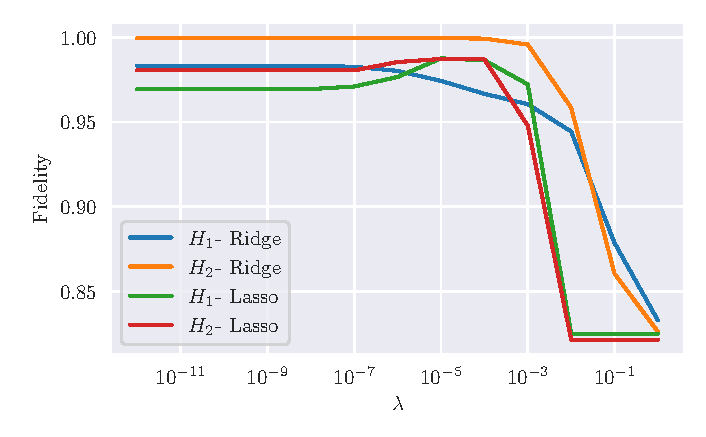
\includegraphics{figures/without_rz_ab_new.pdf}
        \caption{Fidelity as function of lambda for Ridge and Lasso regression}
        \label{fig:fidelity_vs_lmb}
    \end{center}
\end{figure}


\begin{figure}
    \begin{center}
        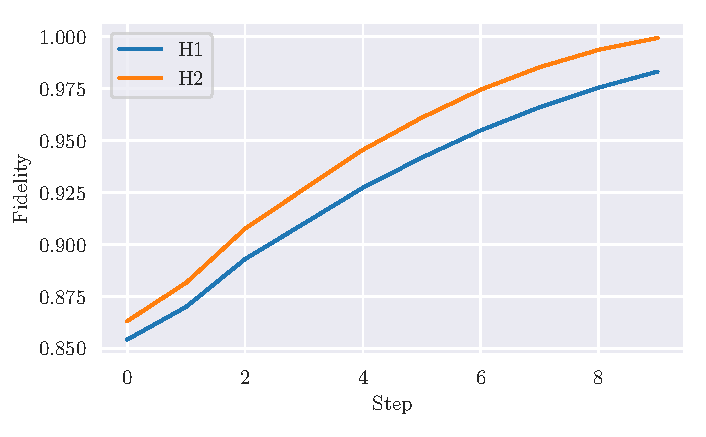
\includegraphics{figures/Fidelity_dynamic_lmb_without_rz_new.pdf}
        \caption{Fidelity as a function of imaginary step}
        \label{fig:nolabel}
    \end{center}
\end{figure}

\section{Generative Learning}
Maybe generative learning should be an own chapter and discriminative learning another one?

\subsection{Parameter investigation}

First step is to find an approximation of where the initial learning rate should be, according to \url{https://arxiv.org/abs/1506.01186} it is possible to increase the learning rate and choose the learning rate which gives the largest decrease in loss. keep plotting until the loss is 4 times larger than then largest loss. Due to this not being distintive data but rather training on the same data, we use this method to find an approximative of where the learning rate should be in further investigations.

\begin{figure}%
    \centering
    \hspace*{-0.1\textwidth}
    \subfloat[\centering]{{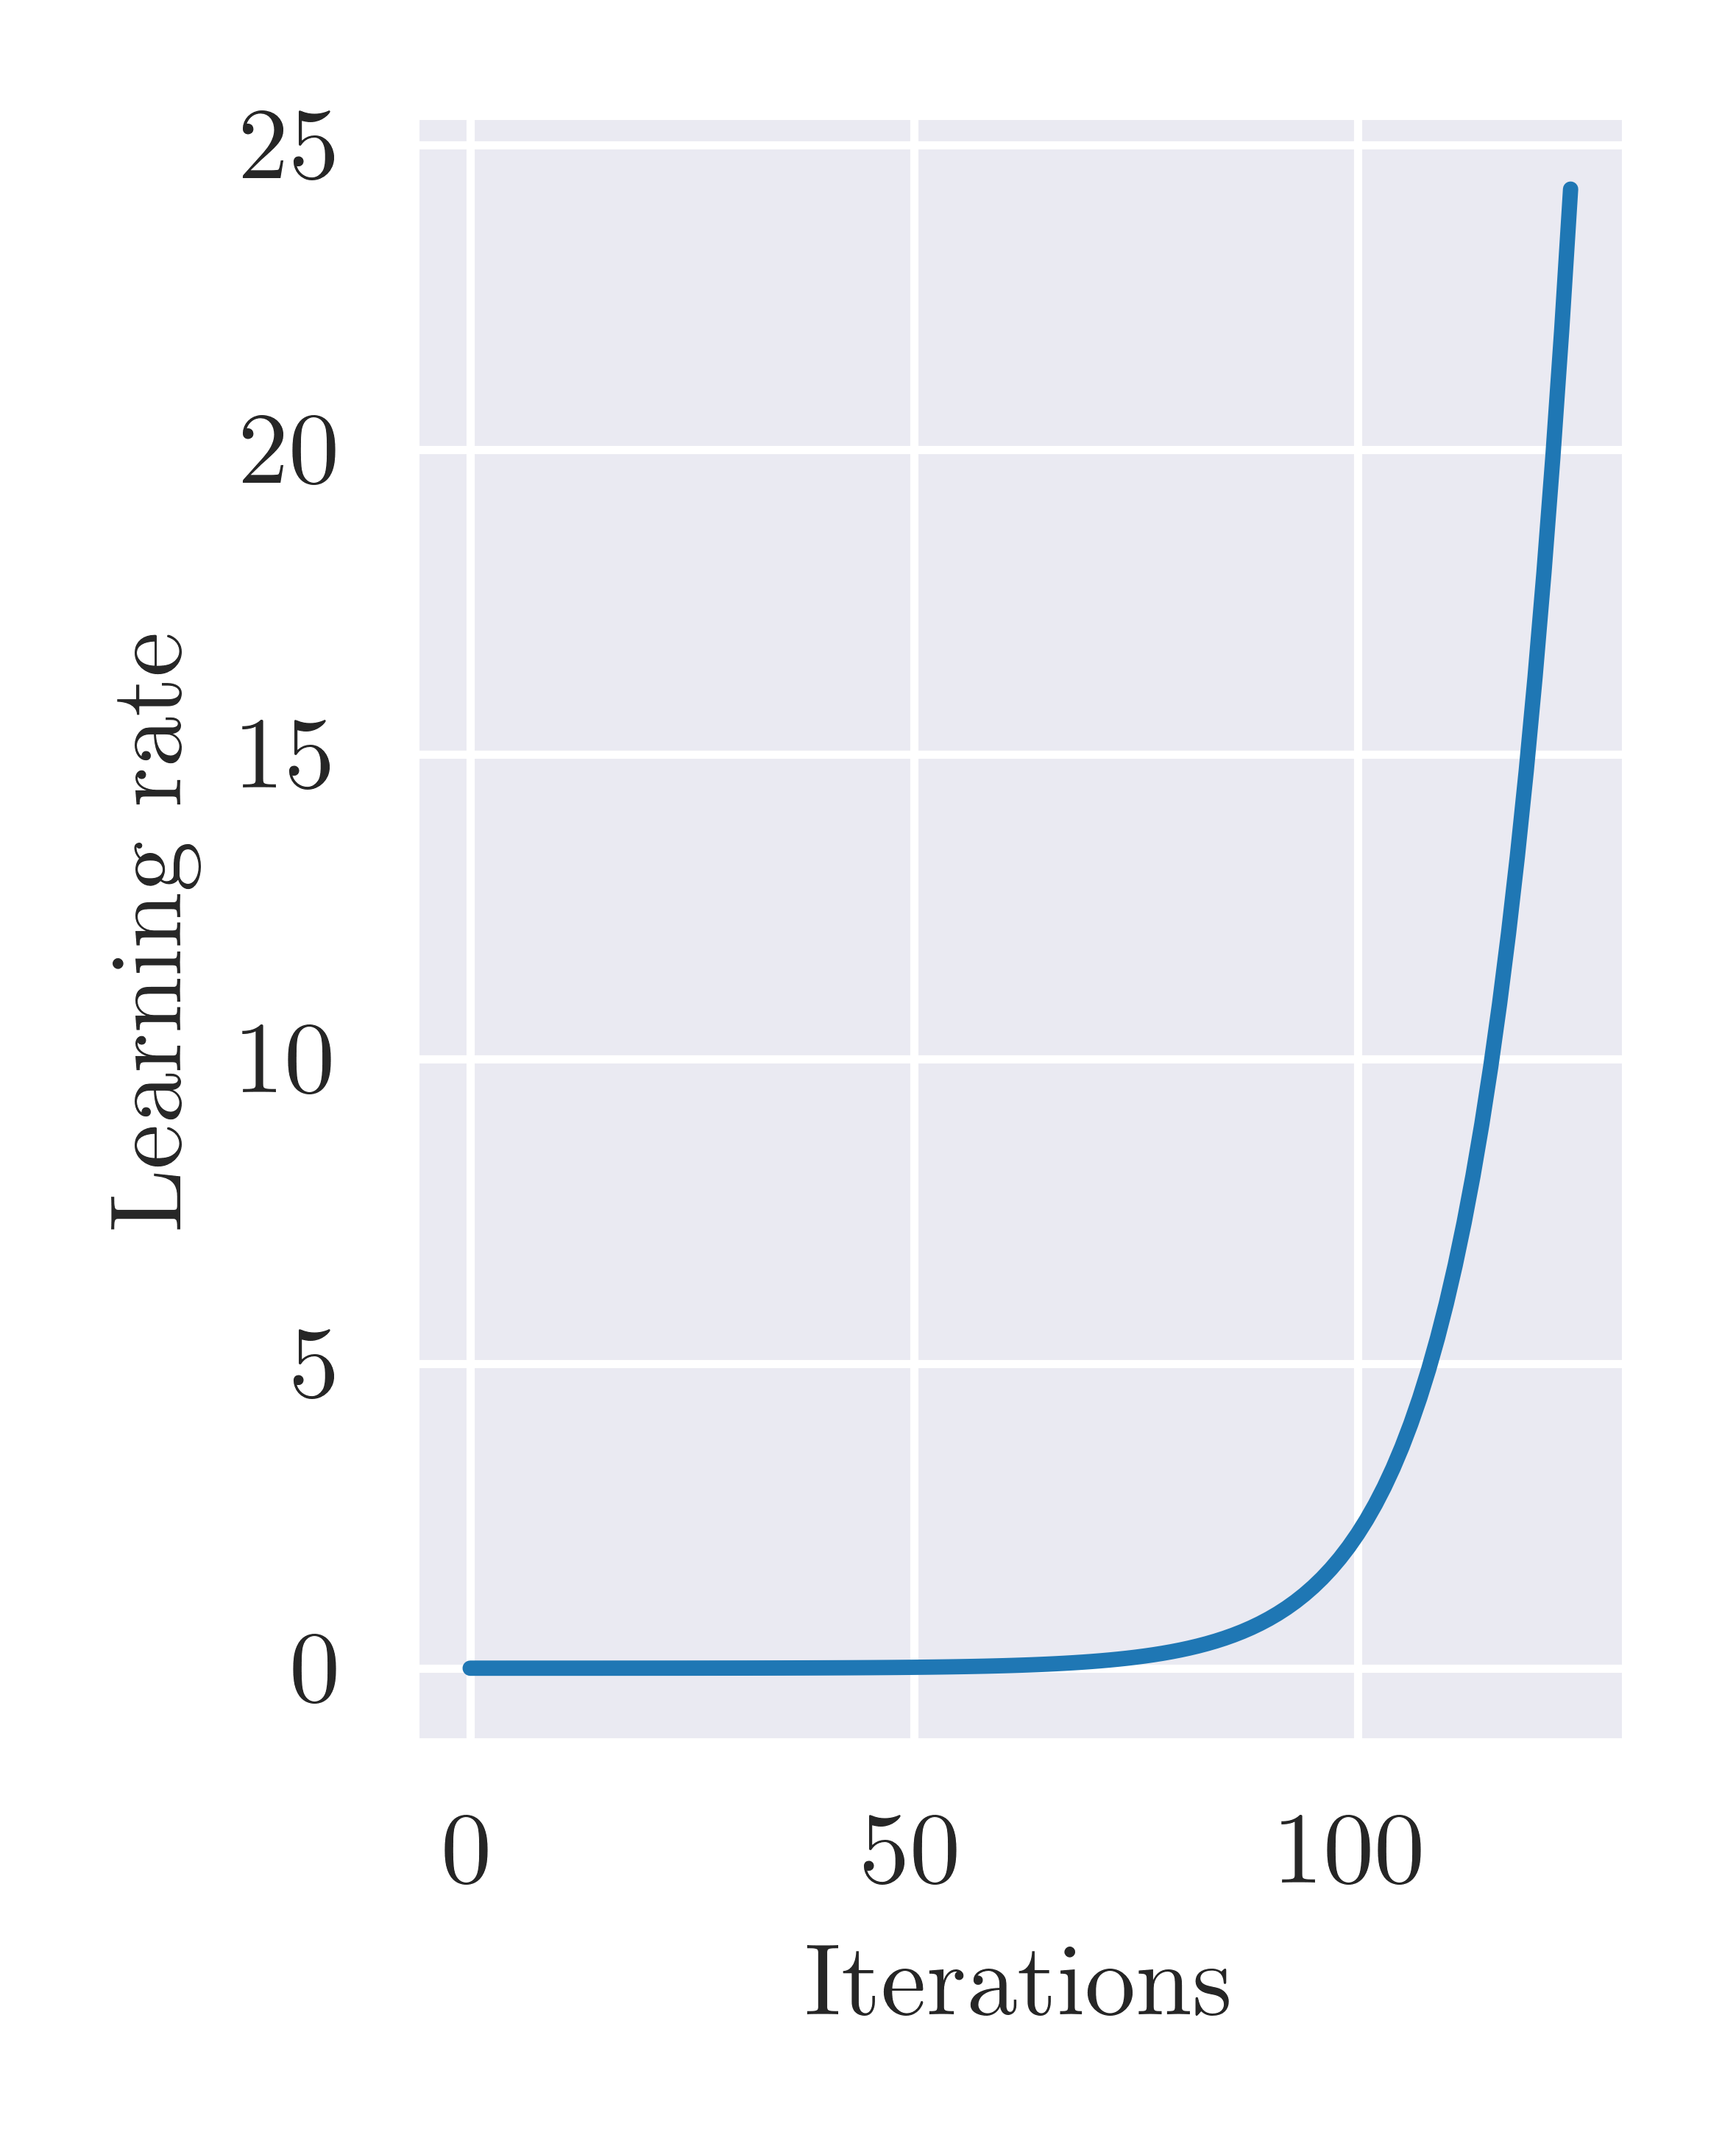
\includegraphics[width=0.6\textwidth]{figures/SGDitVSloss_hs.png} }}%
    %\qquad
    \subfloat[\centering]{{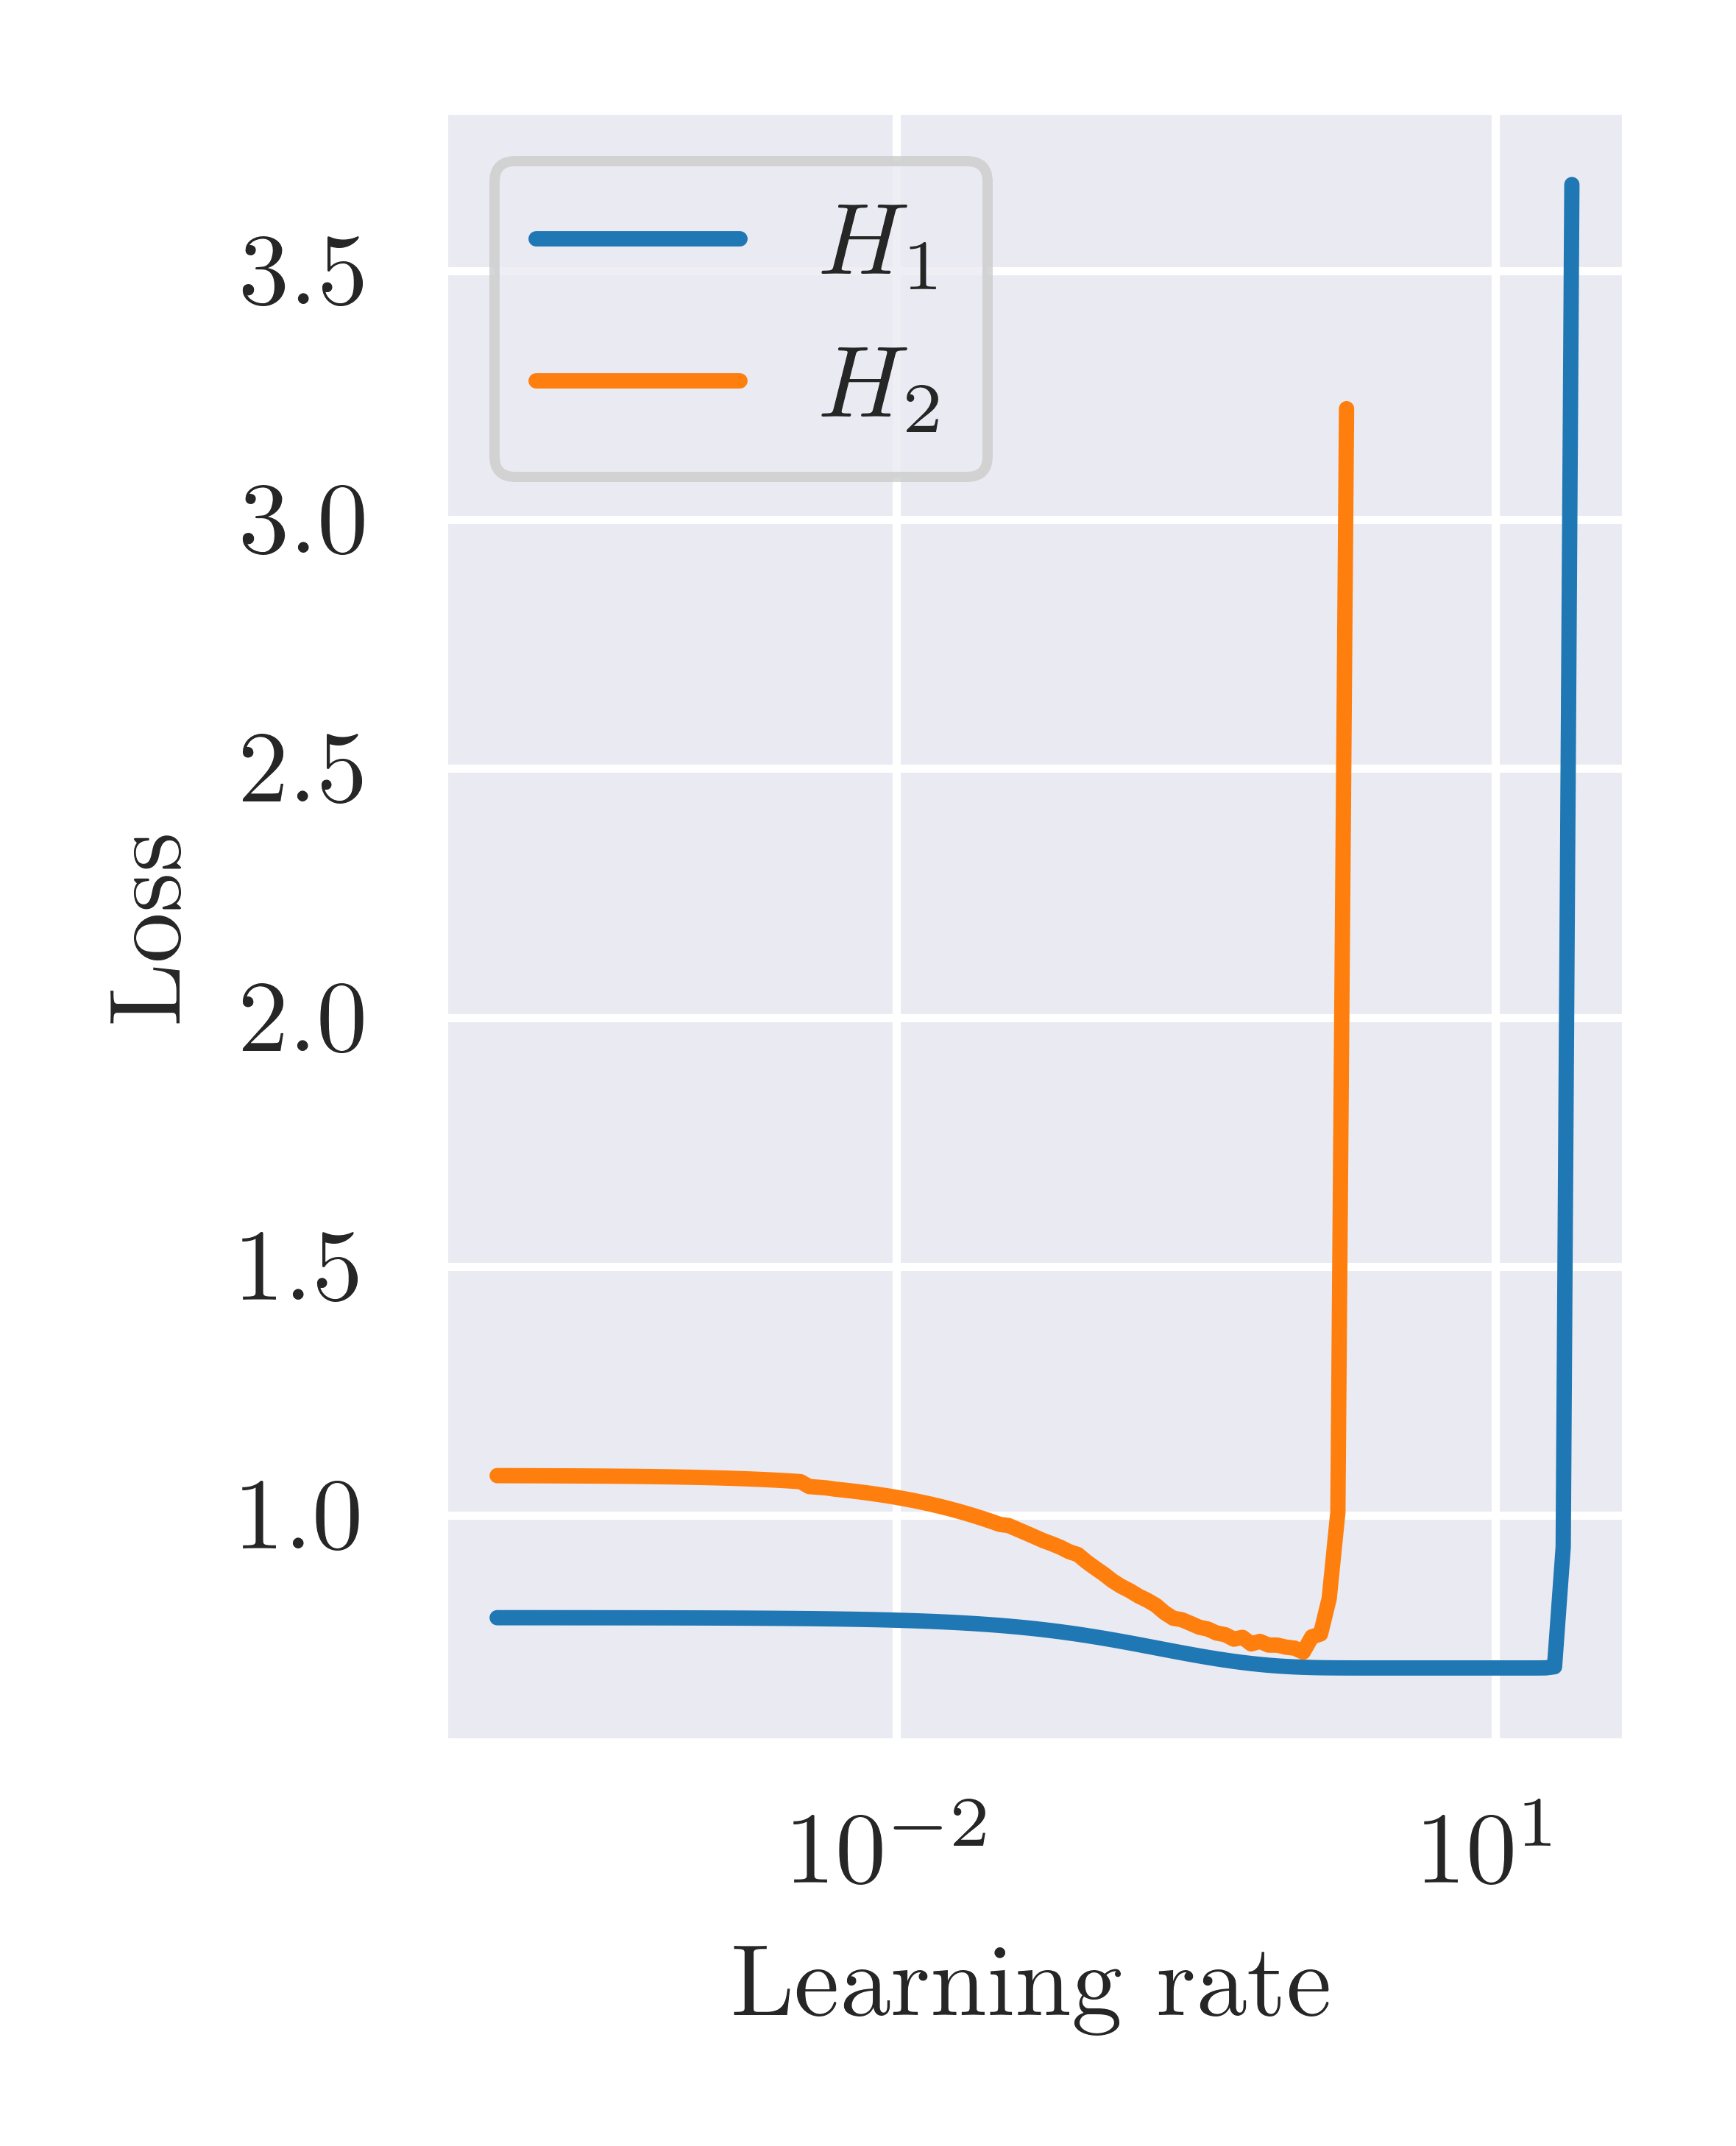
\includegraphics[width=0.6\textwidth]{figures/SGDlrVSloss_exp_SGDitVSloss_hs.png} }}%
    \caption{Optimal learning rate (largest negative derivative= 0.22~0.2 as initial learning rate. a) Increament of learning rate applied to figure b). b) Loss as a function of increased learning rate}%
    \label{fig:lr_exp}%
\end{figure}

\autoref{fig:lr_exp} argues that the optimal learning rate lays in the range of $0.2$. Figure \autoref{fig:H1_loss_es} shows how the learning rates and optimization technique applies to a $1$ qubit Hamiltonian.

\begin{figure}
    \begin{center}
        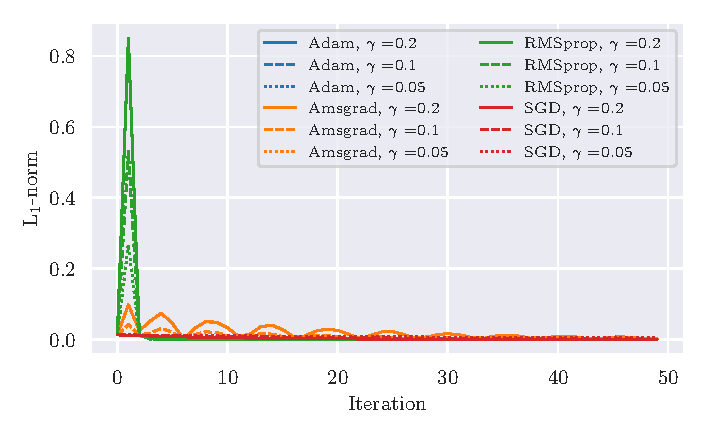
\includegraphics{figures/H1_ab_new_norm.pdf}
        \caption{Generating a probability distribution using a 1 qubit Hamiltonian. Good initialisation, using norm instead of loss due to being easier to notice the trend}
        \label{fig:H1_loss_es}
    \end{center}
\end{figure}

\begin{figure}
    \begin{center}
        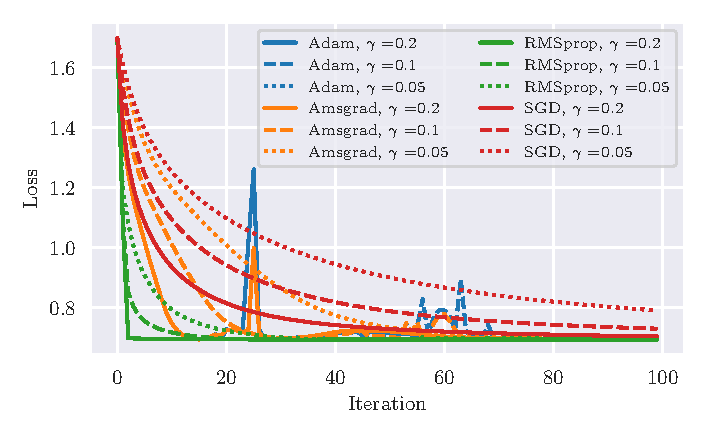
\includegraphics{figures/H2_ab_loss_linear.pdf}
        \caption{2 qubit Hamiltonian, reproducing the Bell state. Loss as a function of iterations for different optimization methods and learning rates, recreating a Bell state. The ADAM optimizer overlaps mostly with the AMSGrad optimizer.}
        \label{fig:loss_vs_it_vs_lr}
    \end{center}
\end{figure}

\autoref{fig:loss_vs_it_vs_lr} indicates that the optimal optimizer of the ones tested is RMSprop. Learning rate of 0.1 is chosen due to H1 0.2 blowing up. \autoref{fig:rms_m} shows how the momentum affects the optimization.

\begin{figure}
    \begin{center}
        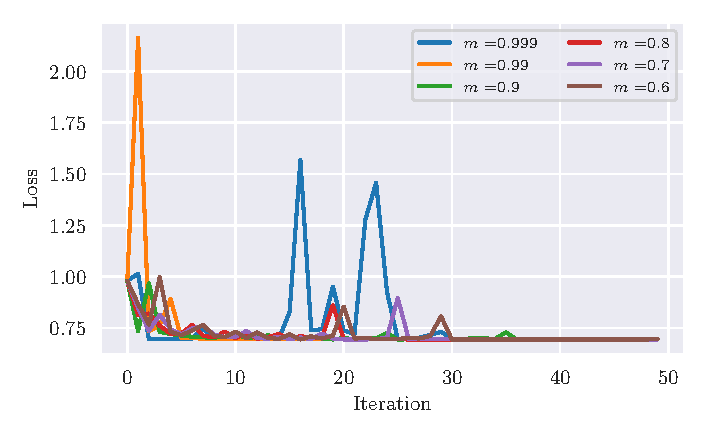
\includegraphics{figures/H2_rms_search_ab_loss_notlog.pdf}
        \caption{Loss as a function of iteration using RMSprop with different initial momentum and learning rate 0.1.}
        \label{fig:rms_m}
    \end{center}
\end{figure}

\subsection{Generating probability distributions}

\begin{figure}
    \begin{center}
        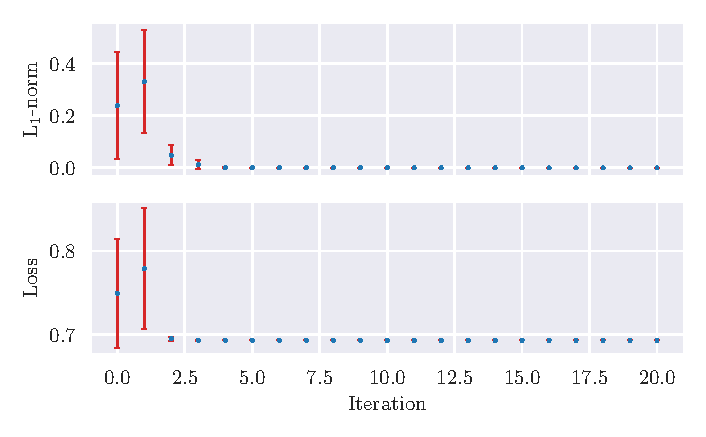
\includegraphics{figures/H1_ab_sub_10seeds.pdf}
        \caption{Generation of a probability distribution [0.5, 0.5] using a 1 qubit Hamiltonian. The quantum Boltzmann machine is fully visible. Loss and norm as a function og iteration steps. The plot represents the mean of 10 random seeds, and the bars represent the standard deviation.}
        \label{fig:nolabel}
    \end{center}
\end{figure}

\begin{figure}
    \begin{center}
        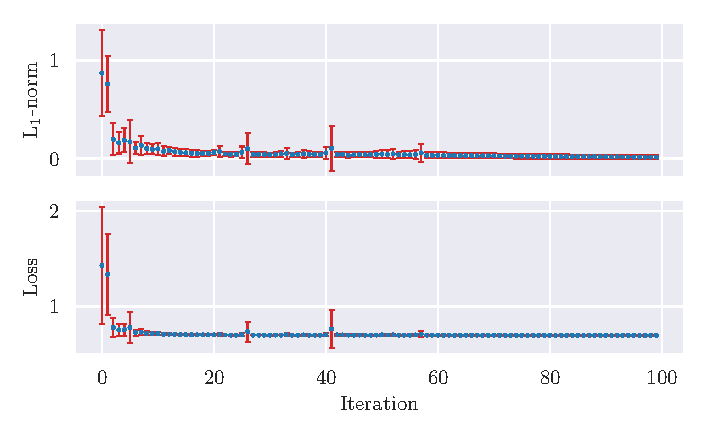
\includegraphics{figures/H2_ab_sub_10seeds.pdf}
        \caption{Too hard to see? Generation of a 2 qubit Hamiltonian. The quantum Boltzmann machine is fully visible. Loss and norm as a function of iteration steps. The plot represents the mean of 10 random seeds, and the bars represent the standard deviation.}
        \label{fig:nolabel}
    \end{center}
\end{figure}

\begin{figure}
    \begin{center}
        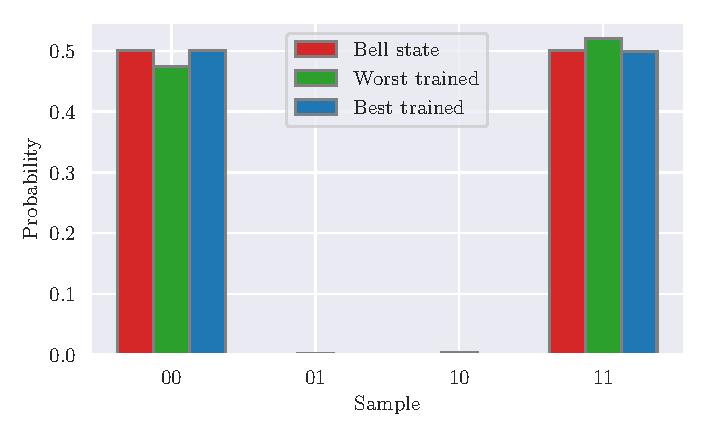
\includegraphics{figures/H2_abRMS_lr01m099bar_10seeds.pdf}
        \caption{Seems good}
        \label{fig:nolabel}
    \end{center}
\end{figure}

\section{Discriminative Learning-Transaction dataset}
This section contains results regarding discriminative learning. Where The fraud dataset and 8x8 MNIST dataset were used.

\subsection{VarQBM: Input as bias}
In this section the input of the VarQBM were inserted according to \todo[inline]{Insert referal to the bias input section when the section is done}
\subsection{VarQBM: Neural Network feature engineering}
In this section the input of the VarQBM were inserted according to \todo[inline]{Insert referal to the neural network input section when the section is done}

Starts with initialization of weights in \autoref{fig:init_X_and_H}.

\begin{figure}%
    \centering
    \subfloat[\centering]{{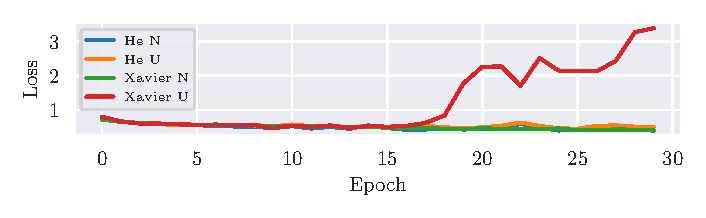
\includegraphics[width=\textwidth]{figures/loss_train12_2_sig_initialisationhhall.pdf} }}%
    \\
    \subfloat[\centering]{{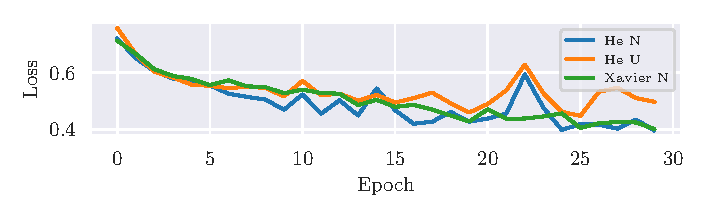
\includegraphics[width=\textwidth]{figures/loss_train12_2_sig_initialisationhh3.pdf} }}%
    \caption{Initialisation of weights. N is normal, U is uniform a) 4 different initialisations b) A better view of He normal, He uniform and Xavier normal}%
    \label{fig:init_X_and_He}%
\end{figure}

\begin{comment}
\begin{figure}
\centering
\begin{subfigure}[\centering]
   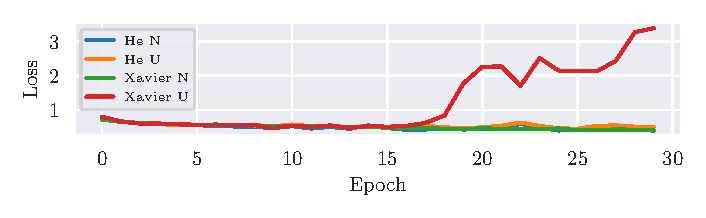
\includegraphics[width=1\textwidth]{figures/loss_train12_2_sig_initialisationhhall.pdf}
   \caption{}
  \end{subfigure}
\begin{subfigure}[\centering]
   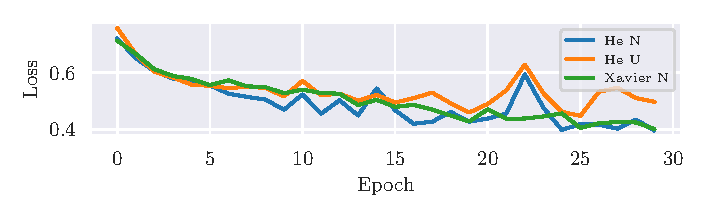
\includegraphics[width=1\textwidth]{figures/loss_train12_2_sig_initialisationhh3.pdf}
   \caption{}
\end{subfigure}
\caption{Le caption}
\end{figure}
\end{comment}

\begin{figure}%
    \centering
    \subfloat[\centering]{{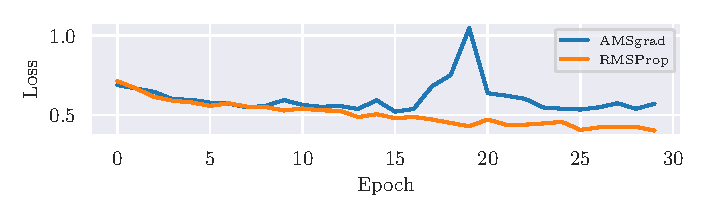
\includegraphics[width=\textwidth]{figures/loss_trainsig_12_2_lroptim_subH2.pdf} }}%
    \\
    \subfloat[\centering]{{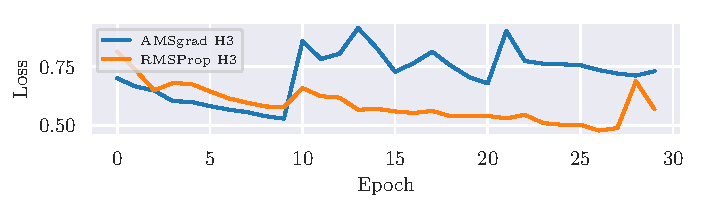
\includegraphics[width=\textwidth]{figures/loss_trainsig_12_2_lroptim_sub_H3.pdf} }}%
    \caption{Tested both H2 and H2.2 with AMSgrad and RMSProp, might remove this, cause it is not that relevant and but we'll what ends up in the thesis eventually.}%
    \label{fig:lr_exp}%
\end{figure}

\begin{figure}
    \begin{center}
        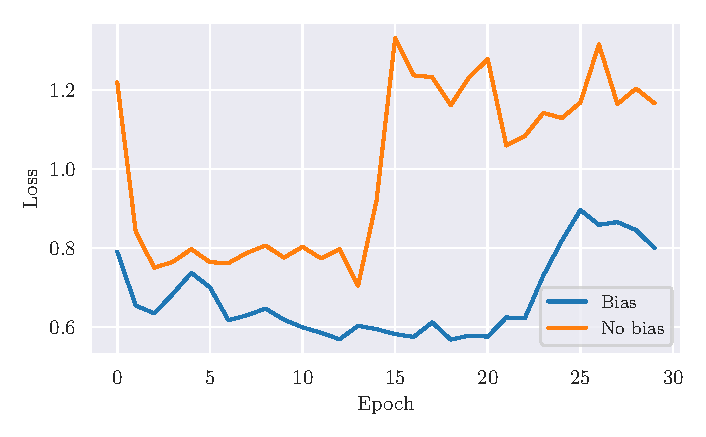
\includegraphics{figures/bias_12_2_50_samples.pdf}
        \caption{2 hidden layers with 12 hidden nodes each and sigmoid activation functions within the hidden layers, with and without bias initialized as 0.01 using 50 samples. The neural net is initialized using xavier normal initialisation.}
        \label{fig:4}
    \end{center}
\end{figure}

\begin{figure}
    \begin{center}
        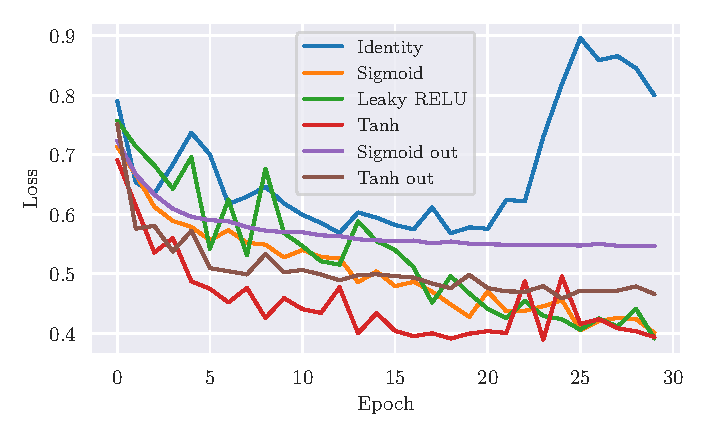
\includegraphics{figures/loss_activations_12_2_without_relu.pdf}
        \caption{2 qubit Hamiltonian with 1 hidden qubit, using a neural network of 2 hidden layers with 12 hidden nodes and bias, using 50 samples, computed using different activation functions.}
        \label{fig:3}
    \end{center}
\end{figure}


\begin{figure}
    \begin{center}
        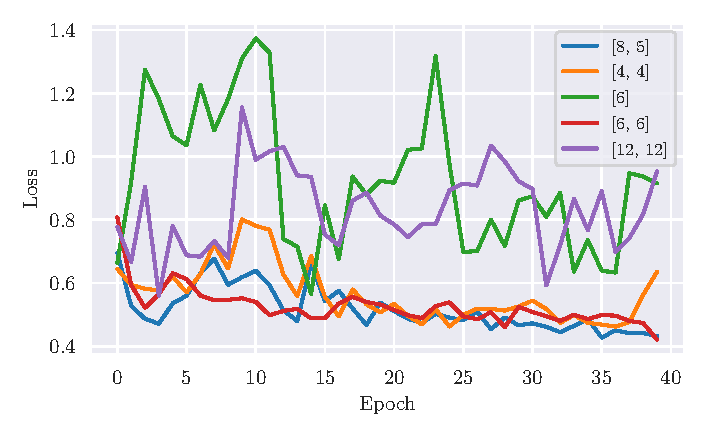
\includegraphics{figures/H2_NNsizes_tr_fraud.pdf}
        \caption{Layer sizes- Transaction dataset. 100 samples in all plots below}
        \label{fig:2}
    \end{center}
\end{figure}

\begin{figure}
    \begin{center}
        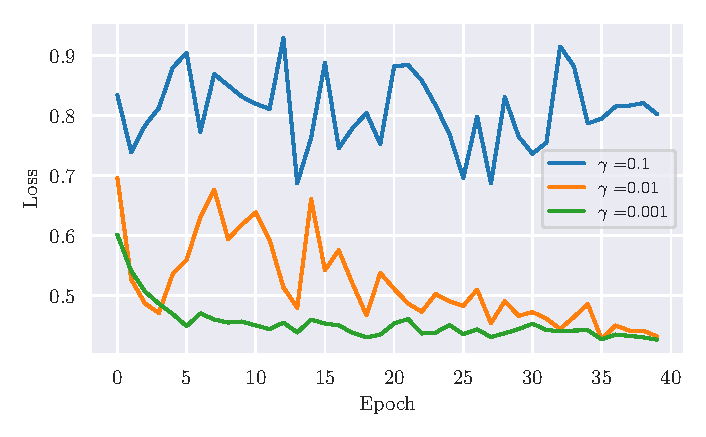
\includegraphics{figures/H2_lr_fraud_tr.pdf}
        \caption{Learning rate- Transaction dataset}
        \label{fig:1}
    \end{center}
\end{figure}

\subsection{Restricted Boltzmann machine}
Solving the transaction data using a restricted Boltzmann machine with logistic regression layer on top.

First set the amount of hidden nodes. The accuracy were plotted as a function of hidden nodes using default values of scikit-learn. Here all samples were labeled as non fraud, so 30 hidden nodes were chosen.

Then an exhaustive search over specified parameter values were done searching across the following values:

\begin{center}
\begin{tabular}{l l}
 Learning rate: & 0.001, 0.005, 0.01, 0.05, 0.1, 0.5 \\ 
 Batch size & 1, 2, 5, 10  \\  
 Logistic hyperparameter C & 0.5, 1, 5, 10, 50, 100, 500    
\end{tabular}
\end{center}

Best parameters found from grid search performed was learning rate of 0.001, batch size of 1 and hyperparameter C 0.5.

The cofusion matrix can be seen in \autoref{fig:transaction_cm}. Easy to see that the RBM still labels all samples as fraud.
\begin{figure}
    \begin{center}
        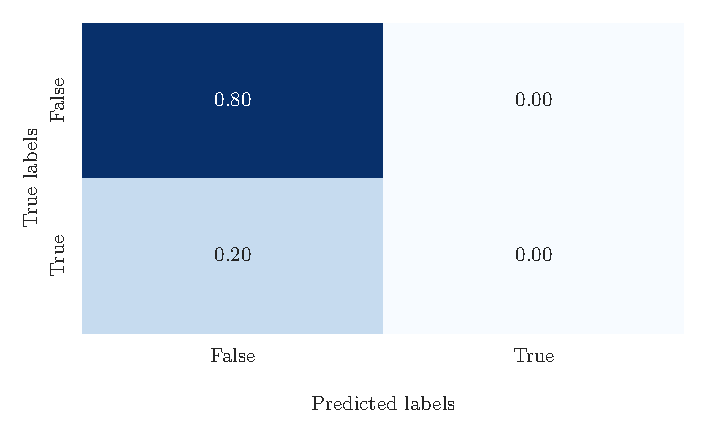
\includegraphics{figures/CMfraud.pdf}
        \caption{RBM- confusion matrix- Transactions. All samples are classified as fraud}
        \label{fig:transaction_cm}
    \end{center}
\end{figure}

\subsection{Transaction data scores}
The final runs achieved using the classical RBM and the VarQBM with and without neural network feature engineering can be seen in \autoref{tab:final_results_table_transaction}

\begin{table}[H]
\centerline{
\begin{tabular}{ ccccc } 
\toprule
 Model & Accuracy & Precision & Recall & $F_1$ score\\ 
\midrule
 VarQBM bias encoding & 0.69 & 0.76 & 0.69 & 0.71 \\
 \textbf{VarQBM NN encoding} &  \textbf{0.82} & \textbf{0.81} & \textbf{0.82} & \textbf{0.78} \\
 RBM &  0.80 & 0.64 & 0.80 & 0.71\\ 
\bottomrule
\end{tabular}}
\caption{Final results, 400 samples, 50 epochs, 0.01}
\label{tab:final_results_table_transaction}
\end{table}

\section{Discriminative Learning-Handwritten image recognition}

Choosing to continue with some of the found parameters from the transaction investigation. Including a bias, if it is better without a bias in the network, it will reduce to 0 during training. In addition the Xavier N initialisation and tanh as activation function within the network are used.

\subsection{VarQBM: Input as bias}
\todo[inline]{Run computations when input is inserted the normal way}
\subsection{VarQBM: Neural Network feature engineering}

\begin{figure}
    \begin{center}
        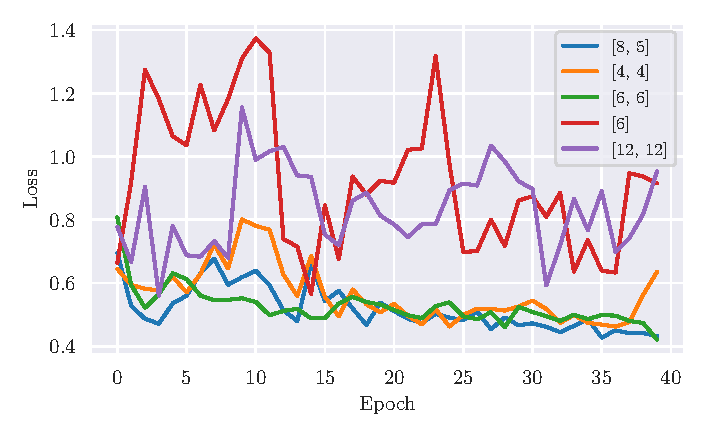
\includegraphics{figures/H2_NNsizes_tr.pdf}
        \caption{Layer sizes- Digit dataset}
        \label{fig:loss_epoch_layers}
    \end{center}
\end{figure}

\begin{figure}
    \begin{center}
        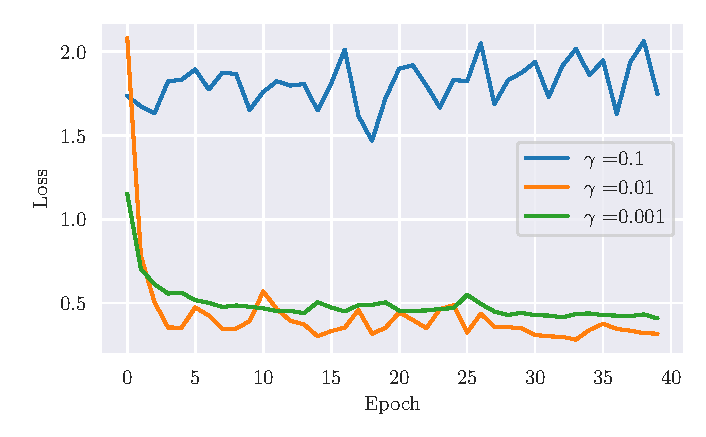
\includegraphics{figures/H2_lr_mnist_tr.pdf}
        \caption{Learning rate- Digit dataset}
        \label{fig:loss_ep_gamma}
    \end{center}
\end{figure}

\subsection{Restricted Boltzmann machine}
Solving the digit dataset using a restricted Boltzmann machine with logistic regression layer on top.

First set the amount of hidden nodes. The accuracy were plotted as a function of hidden nodes using default values of scikit-learn. The results cn be seen in figure \autoref{fig:hn_vs_acc}. The choosen amount of hidden nodes was 30.

\begin{figure}
    \begin{center}
        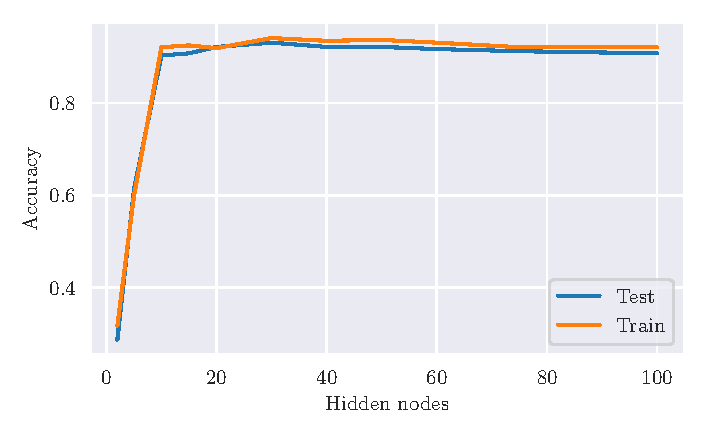
\includegraphics{figures/rbm_h_vs_acc_digit2.pdf}
        \caption{RBM - Accuracy as a function of the number of hidden nodes- Transactions}
        \label{fig:hn_vs_acc}
    \end{center}
\end{figure}

Then an exhaustive search over specified parameter values were done searching across the same values as for the transaction dataset in \todo[inline]{Add referral to the table of gridsearch parameters}

Best parameters found from grid search performed was learning rate of 0.05, batch size of 2 and hyperparameter C of 100.

The cofusion matrix can be seen in \autoref{fig:digit_cm}.
\begin{figure}
    \begin{center}
        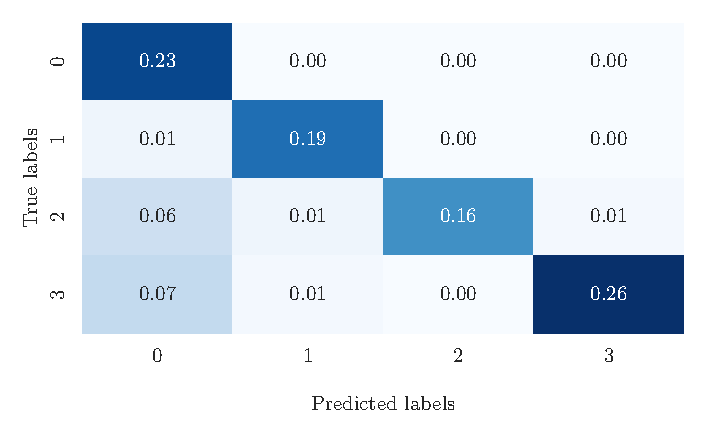
\includegraphics{figures/CMmnist.pdf}
        \caption{RBM- confusion matrix- Digit dataset. }
        \label{fig:digit_cm}
    \end{center}
\end{figure}

RBM with $0.99$ accuracy on digit dataset(Only four classes.

\subsection{Handwritten image recognition scores}
The final runs achieved using the classical RBM and the VarQBM with and without neural network feature engineering can be seen in \autoref{tab:final_results_table_digits}

\begin{table}[H]
\centerline{
\begin{tabular}{ ccccc } 
\toprule
 Model & Accuracy & Precision & Recall & $F_1$ score\\ 
\midrule
 VarQBM bias encoding & 0.56 & 0.54 & 0.56 & 0.53 \\
 VarQBM NN encoding &  0.73 & 0.85 & 0.73 & 0.65 \\
 \textbf{RBM} &  \textbf{0.98} & \textbf{0.98} & \textbf{0.98} & \textbf{0.98} \\
\bottomrule
\end{tabular}}
\caption{Final results, 400 samples, 50 epochs, 0.1lr. weighted precision, recall and F1 score, NN layer: [8,5]}
\label{tab:final_results_table_digits}
\end{table}

\section{MNIST scores}
The final runs achieved using the classical RBM and the VarQBM with neural network feature engineering can be seen in \autoref{tab:final_results_table_mnist}
\begin{table}[H]
\centerline{
\begin{tabular}{ cccccc } 
\toprule
 Model & NN encoding &Accuracy & Precision & Recall & $F_1$ score\\ 
\midrule
 VarQBM & [32,32]& 0.83 & 0.86 & 0.83& 0.84 \\
 VarQBM & [123,19] & 0.33 & 0.11 & 0.33 & 0.16 \\
 \textbf{RBM} & & \textbf{0.91} & \textbf{0.91} & \textbf{0.91} & \textbf{0.91} \\
\bottomrule
\end{tabular}}
\caption{28x28 pixels, 4 classes. Final results, 400 samples, 50 epochs, 0.01lr. weighted precision, recall and F1 score}
\label{tab:final_results_table_mnist}
\end{table}



\end{document}